\documentclass[titlepage,a4paper]{jsarticle}
\usepackage{../sty/import}% 各種パッケージインポート
\usepackage{../sty/title}% タイトルページの変更

%% タイトルページの変数
% レポートタイトル
\title{環境経済学期末試験}
% 提出日
\expdate{\today}
% 科目名
\subject{環境経済学}
% 分野
\class{情報経営システム工学分野}
% 学年
\grade{B3}
% 学籍番号
\mynumber{24336488}
% 記述者
\author{本間三暉}

\begin{document}
% titleページ作成
\maketitle
\section{記述問題}
\subsection*{国際交渉の結果、ある国が二酸化炭素排出量をXトン削減する義務を負うことになった。
  そこで、 図\ref{環境図}のとおり、政府は、Raの限界削減コスト曲線を持つ企業Aに、Xaトンの削減量を、Rbの限界削減 コスト曲線を持つ企業Bに、Xbトンの削減量を割り当てたとする。
  ただし、X=Xa+Xbと仮定する。}
\begin{figure}[H]
  \centering
  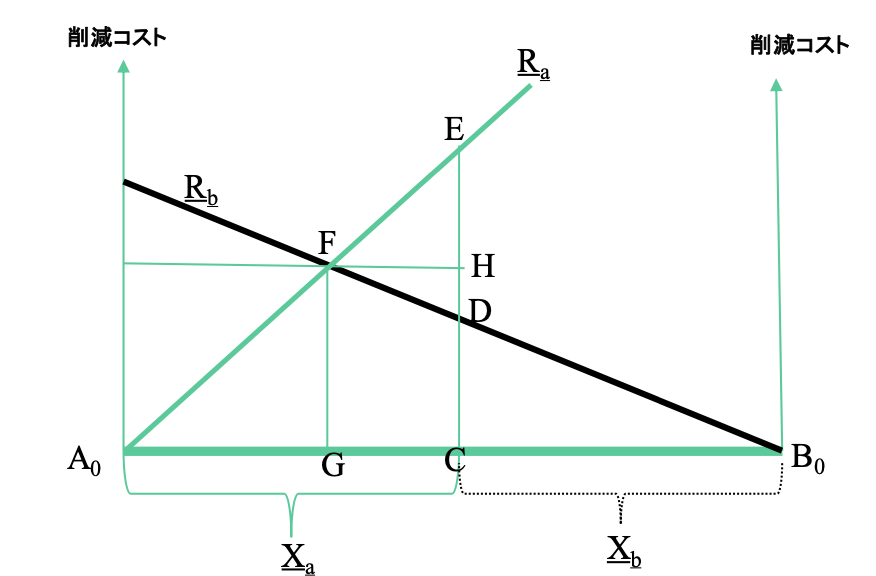
\includegraphics[width=12cm]{img/env.png}
  \caption{環境図}
  \label{環境図}
\end{figure}

\subsection{二酸化炭素削減量取引を許さない場合の削減コストを求めよ。}\label{問一}
図\ref{環境図}より,企業Aの削減コストが$\triangle A_0CE$,企業Bの削減コストが$\triangle B_0CD$なので,
二酸化炭素削減量取引を許さない場合の全体の削減コストは式\eqref{1:削減コスト}に示す通り,$\square A_0EDB_0$となる.
\begin{align}
  \triangle A_0CE + \triangle B_0CD = \square A_0EDB_0 \label{1:削減コスト}
\end{align}

\subsection{二酸化炭素削減量取引を許す場合の削減コストを求めよ。}\label{問二}
図\ref{環境図}より,企業Aの削減コストが$\triangle A_0FG$,企業Bの削減コストが$\triangle B_0FG$なので,
二酸化炭素削減量取引を許す場合の全体の削減コストは式\eqref{2:削減コスト}に示す通り,$\triangle A_0FB_0$となる.
\begin{align}
  \triangle A_0FG + \triangle B_0FG = \triangle A_0FB_0 \label{2:削減コスト}
\end{align}

\subsection{二酸化炭素削減量取引を許す場合と許さない場合の削減コストを比較せよ。}
図\ref{環境図}と節\ref{問一},\ref{問二}より,炭素削減量取引を許す場合は許さない場合に比べ式\eqref{3:差分}に示す通り,コストは$EFD$減少する.
\begin{align}
  \square A_0EDB_0 - \triangle A_0FB_0 = \triangle DEF\label{3:差分}
\end{align}
次に,$CG$分がB社からA社に単品価格$H$で販売されるので,販売額は$\square FHCG$となる.
この取引からB社は,販売収入$\square FHCG$から生産コスト$\square FDCG$を差し引いた$\triangle HDF$分の利益を上げる.
また,A社は取引を通じて,$\square GCEF$分の生産コストを削減し,そのうちの$\square FHGC$分を取引代金としてB社に支払うが,
残りの$\triangle FEH$分は避けられたコストであり,利益増加分に等しい.
よって,取引することで取引しないときに比べ,削減コストが$\triangle HEF$少なくなる.
\subsection{二酸化炭素削減量取引を許す場合の、取引量、取引価格を求めよ。}
取引量は$R_a$と$R_b$の交点から削減量までの部分に相当するので$CG$,取引価格は$R_a$と$R_b$の交点までの高さに相当するので$FG$となる.

\section{レポート課題}
\subsection*{道路輸送部門の脱炭素化を実現するために、自動車の電動化が必要不可欠である。
  自動車電動化の推進にどのような対策が必要か、ZEV(Zero Emission Vehicle)目標規制・クレジット取引制度をどう位置づけるか 等について、検討せよ。}
  
% 参考文献
\begin{thebibliography}{99}
  \bibitem{}
\end{thebibliography}

\end{document}